% Star tracker-accelerometro-gps
Esistono diversi tipi di sensori per la determinazione dell'assetto e
dell'orbita del satellite.
\begin{itemize}
\item Sensori inerziali: come accelerometri o giroscopi, sensibili alla causa
del movimento
\item Sensori d'assetto: come i magnetometri, gli star trackers o i GPS,
osservano il moto
\item Sensori di posizione: come i GPS, individuano la posizione dello strumento
\end{itemize}
Verranno descritti solo i sensori utilizzati ai fini della simulazione.
\paragraph{Accelerometro}
Esso permette di misurare l'accelerazione lineare del centro di massa.
L'implemetazione è realizzata mediante una piccola massa (proof-mass)
all'interno di una scatola, che la protegge dalle
forze esterne cui è soggetto il satellite. Per fare ciò, è necessario che il
satellite insegua la massa, o che la massa insegua il satellite. La proof-mass
è soggetta alla sola forza gravitazionale, quindi è in caduta libera,
ciò implica che la forza utilizzata per mantenere la massa di prova ferma
rispetto alla scatola che la contiene, può essere utilizzata per misurare le
forze esterne al satellite, vedi figura \ref{fig:accelerometro} \begin{figure}[htp]
\begin{center}
  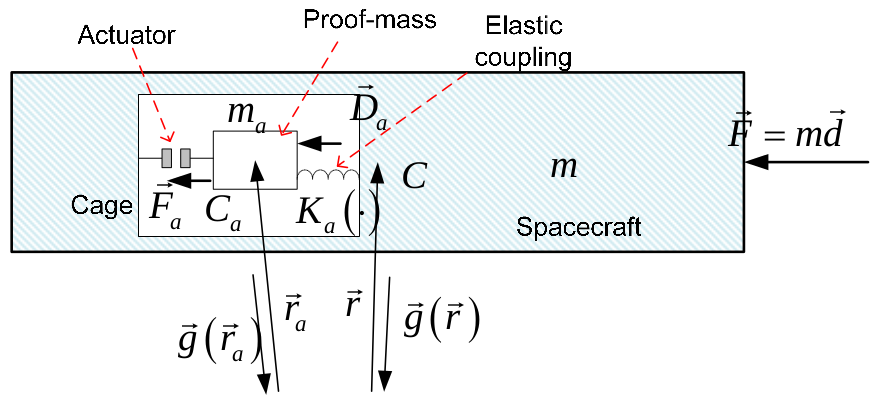
\includegraphics[width=\textwidth]{modelling/attitude_kinematics_and_dynamics/image/accelerometro.png}
  \caption{Massa di prova di un accelerometro}
  \label{fig:accelerometro}
\end{center}
\end{figure}
Indichiamo con $m$ la massa del satellite e con $m_a$ la massa della proof-mass,
$\vec{r}$ e $\vec{v}$ indicano la posizione  e la velocità del satellite, mentre
$\vec{r}_a$ e $\vec{v}_a$ indicano la posizione e la velocità della massa di
prova. Le equazioni di Newton della massa $m_a$ e del satellite sono
\begin{equation}
\dot{\vec{v}}(t)=-\vec{g}(\vec{r}(t))+\frac{\vec{F}(t)-\vec{F}_a(t)}{m}
\end{equation}
\begin{equation}
\dot{\vec{v}}_a(t)=-\vec{g}(\vec{r}_a(t))+\frac{\vec{F}_a(t)}{m_a}+\frac{\vec{D}_a(t)}{m_a}
\end{equation}
dove $\vec{D}_a$ indica le forze parassite agenti sulla proof-mass. Attraverso
la misura di $\vec{F}_a$ è quindi possibile risalire alle forze esterne al
satellite.

Tra gli errori di misura che affliggono le misurazioni effettuate tramite un accelerometro
è presente il bias, cioè un offset sistematico, dovuto alla tecnologia costruttiva, che viene
aggiunto alle misure. Nel controllo, purtroppo, tale errore viene interpretato come disturbo
dall’osservatore che quindi stima il drag sommato alla polarizzazione dell’accelerometro. Per
ovviare a tale difetto si agisce eliminando il valor medio del bias dall’uscita dell’osservatore.
Tuttavia l’orbita non sarà mai priva di accelerazioni non gravitazionali, poiché tra gli errori
dell’accelerometro è presente anche una deriva aleatoria.
